% !TEX root = QlockToo.tex
% Software
\section{Software}
\label{sec:Software}

\begin{figure}[t]
    \centering
    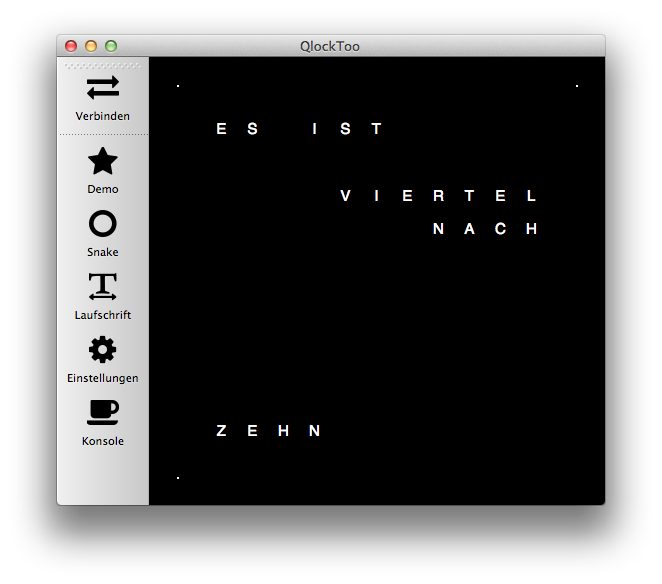
\includegraphics[width=.8\textwidth]{Abbildungen/Manager}
    \caption[QlockToo-Manager]{Der QlockToo-Manager}
    \label{fig:Manager}
\end{figure}

\begin{multicols}{2}
Noch vor der Konzeption der Uhr wird eine Desktop-Software entwickelt, um den Testprozess für die Algorithmen zu beschleunigen. Mit der Zeit wächst der Umfang des Programms jedoch deutlich und es enthält mittlerweile folgende Funktionen:

\begin{itemize}
\item Die QlockToo kann über USB angeschlossen und als Display genutzt werden. Dazu kommt ein selbst entwickeltes Streaming-Protokoll zum Einsatz.
\item Die Software enthält einen Simulator. So können Muster und Algorithmen auch ohne Anschluss an die Hardware getestet werden.
\item Zu Testzwecken sind verschiedene Demonstrationsmuster implementiert
\item Das Spiel Snake kann auf der QlockToo gespielt werden. Die Steuerung erfolgt über die Pfeiltasten am Computer.
\item Es können Laufschriften in beliebiger Geschwindigkeit angezeigt werden.
\item Ein Einstellungsdialog, in dem alle wichtigen Einstellungen an der QlockToo am Rechner vorgenommen werden können.
\end{itemize}

\subsection{Aufbau}
Da die Software auf allen gängigen Plattformen (Windows / Mac OS X / Linux) lauffähig sein soll und wegen der besonders hohen Entwicklungsgeschwindigkeit wird Python als Programmiersprache verwendet.
Das aus der C++ - Welt bekannte Framework Qt wird über die von Digia bereitgestellten PySide -Bindings als GUI-Framework genutzt. Die Software baut somit ausschließlich auf freier Open-Source Software auf.

\subsection{Rundgang durch die Software}
Der QlockToo-Manager zeigt nach dem Start den Simulator und eine seitlich angebrachte Menüleiste zum Starten der Unterprogramme.
Das Programm \emph{Timewords}, welches für die Anzeige der Zeit in Worten zuständig ist, wird standardmäßig angezeigt, wenn keines der Unterprogramme aktiv ist. Der QlockToo-Manager zieht dazu die momentane Systemzeit heran.

Die Unterprogramme sind jeweils einzelne, unabhängige Python-Module -- lassen sich also leicht erweitern.
Der Simulator besitzt die gleiche API wie die Hardware. Die Ausgabe der Programme kann also ohne Anpassungen auf die Hardware gestreamt werden oder im Simulator angezeigt werden (oder beides gleichzeitig).

\subsubsection{Konnektivität}
\begin{figure}[h]
    \centering
    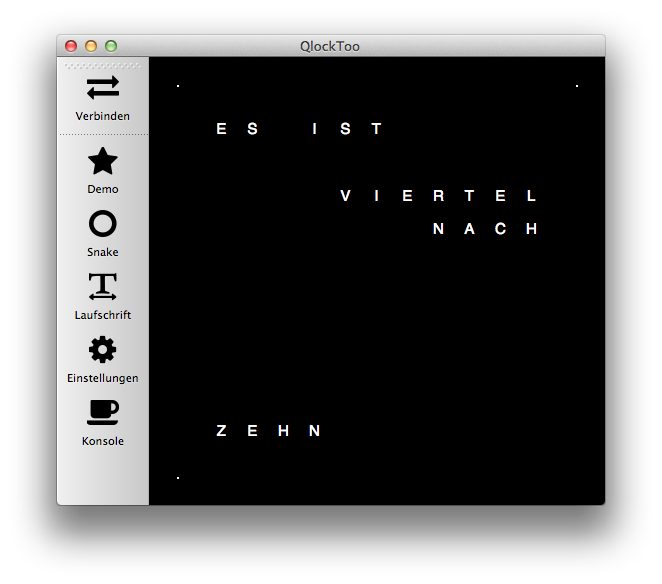
\includegraphics[width=\columnwidth,draft]{Abbildungen/Manager}
    \caption[Verbindungsdialog]{Der Verbindungdialog}
    \label{fig:Verbindungsdialog}
\end{figure}

Für die Entwicklung ist eine Konsole integriert, mit der auf direktem Wege Befehle an die API der QlockToo gesendet werden können. Kommandos und Rückgabewerte werden zur besseren optischen Erfassbarkeit farblich hervorgehoben.
%
\begin{figure}[h]
    \centering
    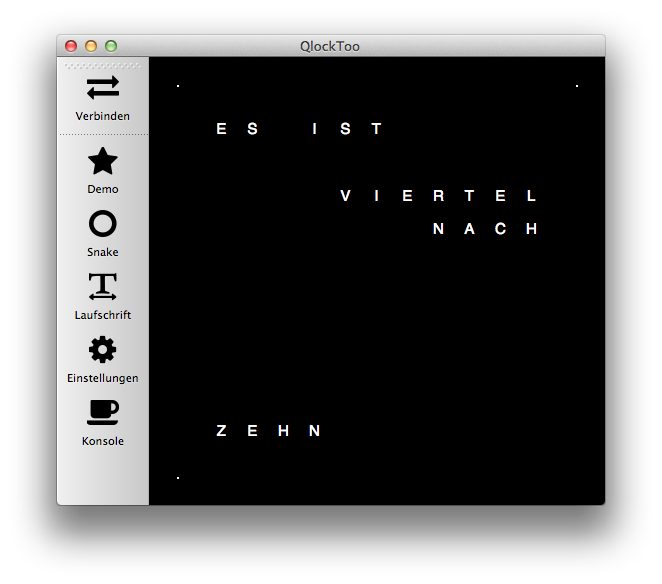
\includegraphics[width=0.9\columnwidth,draft]{Abbildungen/Manager}
    \caption[Konsole]{Die Konsole}
    \label{fig:Konsole}
\end{figure}


\subsubsection{Demonstrationsmuster}
Der nächste Punkt in der Menüleiste sind die Demonstrationsmuster.
Die Abbildungen sind hier zur besseren Sichtbarkeit invertiert dargestellt.

\emph{Pulse} \\
Die Buchstaben und Ecken wechseln sanft zwischen minimaler und maximaler Helligkeit.

\emph{Fade} \\
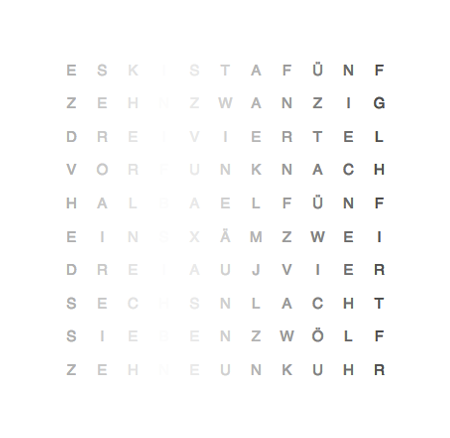
\includegraphics[width=\columnwidth]{Abbildungen/Demo/Fade}
Zeigt einen Farbverlauf auf der Uhr, der sich sinusförmig von links nach rechts und zurück bewegt.

\emph{Wave} \\
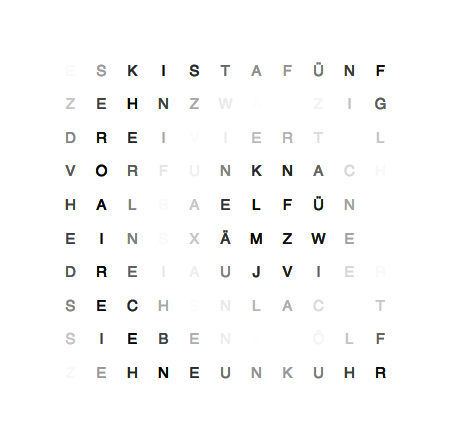
\includegraphics[width=\columnwidth]{Abbildungen/Demo/Welle}
Zeigt ein pulsierendes Wellenbild, dessen Zentrum mit der Zeit langsam wandert.

\emph{Pong} \\
Zeigt zwei perfekt spielende Computergegner bei einer Partie Pong.

\emph{Helix} \\
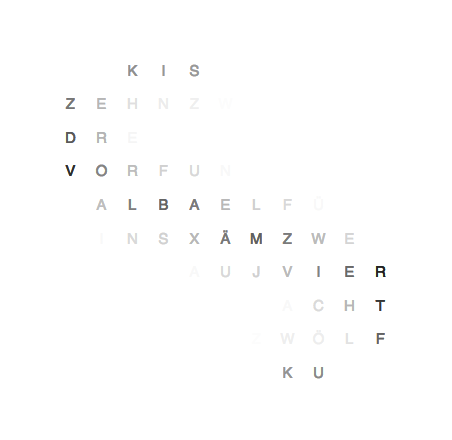
\includegraphics[width=\columnwidth]{Abbildungen/Demo/Helix}
Zeigt die zweidimensionale Projektion einer dreidimensionalen Spirale. Die z-Achse wird dabei über Helligkeitswerte visualisiert.
Bedingt durch die Berechnung der Funktionwerte für diskrete Buchstaben auf der Uhr und die geringe Pixelanzahl der Uhr wirkt die Demonstration zuerst sehr dünn und zerstückelt.
Daraufhin wird ein Gauss-Tiefpass implementiert, der den gewünschten Anti-Alias-Effekt mit sich bringt.

\emph{Game Of Life} \\
Implementation von Conways Spiel des Lebens, wobei tote Zellen schwarz und lebende Zellen weiß dargestellt werden.
Grundlage sind folgende vier Regeln, die bei jeder Iteration befolgt werden\footnote{de.wikipedia.org/wiki/Conways\_Spiel\_des\_Lebens}:
\begin{itemize}
    \item Eine tote Zelle mit genau drei lebenden Nachbarn wird in der Folgegeneration neu geboren.
    \item Lebende Zellen mit weniger als zwei lebenden Nachbarn sterben in der Folgegeneration an Einsamkeit.
    \item Eine lebende Zelle mit zwei oder drei lebenden Nachbarn bleibt in der Folgegeneration lebend.
    \item Lebende Zellen mit mehr als drei lebenden Nachbarn sterben in der Folgegeneration an Überbevölkerung.
\end{itemize}

\emph{Matrix} \\
Der berühmte Effekt aus dem Wachowski-Film \emph{Matrix} bietet sich wegen des Designs der QlockToo besonders an.
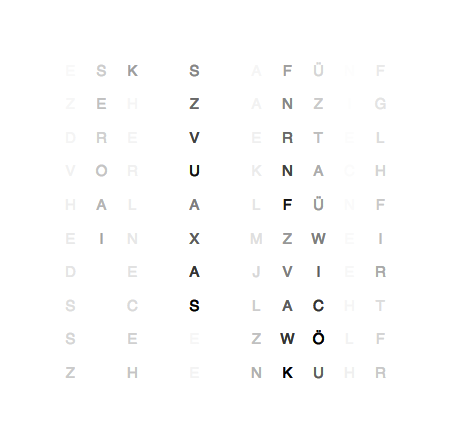
\includegraphics[width=\columnwidth]{Abbildungen/Demo/Matrix}


\end{multicols}

